\documentclass{article}

\usepackage{amsmath}
\usepackage{amssymb}
\usepackage{amsthm}
\usepackage{amsfonts}

\usepackage{tikz}
\usepackage{color}
\usetikzlibrary{calc,shapes,fadings,automata,backgrounds,petri,shapes,decorations,decorations.pathmorphing,decorations.pathreplacing}


\newcommand{\pn}{Petri net}
\newcommand{\pns}{Petri nets}
\newcommand{\apical}{$A\pi$-calculus}
\newcommand{\pical}{$\pi$-calculus}
\newcommand{\nest}{\mathit{nest}_\nu}
\newcommand{\depth}{\mathit{depth}}
\newcommand{\set}[1]{\left\{#1\right\}}
\newcommand{\pset}[2]{\set{\,#1\mid#2\,}}
\newcommand{\process}{\mathcal{P}}
\newcommand{\Reach}{\mathit{Reach}}
\newcommand{\subgraph}{\mathrel{\hookrightarrow}}

\newcommand{\tikzMessage}[1]{
  \draw[thick,fill=white] (#1) rectangle ++(0.6, -0.4);
  \path[draw,-,thick] (#1) -- ++(0.3, -0.2) -- ++(0.3, 0.2); 
}
\newcommand{\tikzMessageNode}[2]{
  \node[draw,thick,fill=white,rectangle,inner sep=0pt,minimum height=0.4cm,minimum width=0.6cm] (#1) at (#2) {};
  \path[draw,-,thick] (#2) -- ++(-0.3, 0.2) (#2) -- ++(0.3, 0.2); 
}

\begin{document}
  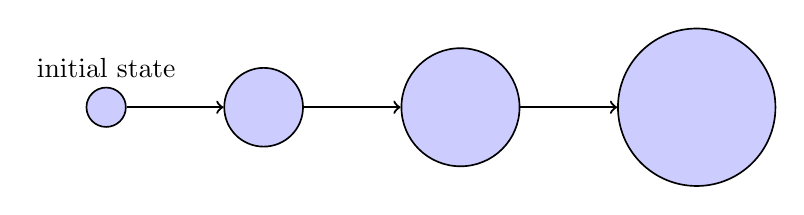
\begin{tikzpicture}[semithick, ->, node distance=2cm]

  \node[draw,circle,fill=blue!20,minimum height=0.5cm]  (init) at ( -4, 0) {};
  \node (initlabel) at ( -4, 0.5) {initial state};
  \node[draw,circle,fill=blue!20,minimum height=1cm]  (s1) at ( -2, 0) {};
  \path[thick] (init) edge (s1);
  \node[draw,circle,fill=blue!20,minimum height=1.5cm]  (s2) at ( 0.5, 0) {};
  \path[thick] (s1) edge (s2);
  \node[draw,circle,fill=blue!20,minimum height=2cm]  (s3) at ( 3.5, 0) {};
  \path[thick] (s2) edge (s3);
  %\node[draw,circle,fill=red!20,minimum height=0.5cm]  (err2) at ( 3.8, -0.5) {};
  \end{tikzpicture}
  
  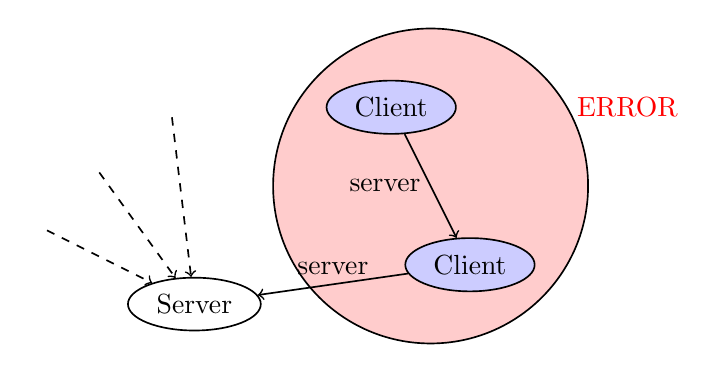
\begin{tikzpicture}[semithick, ->, node distance=2cm]

  \node[draw,circle,fill=red!20, minimum height=4cm] (err1) at (-0.5,1) {} ;
  \node[color=red] (errlabel) at ( 2, 2) {ERROR};
  \node [draw,ellipse,fill=blue!20]  (x) at ( 0, 0) {Client};
  \node [draw,ellipse,fill=blue!20] (ni) at (-1, 2) {Client};
  \path  (ni) edge node [left] {server} (x);
  \node [draw,ellipse]  (server) at ( -3.5, -0.5) {Server};
  \path  (x) edge node [above] {server} (server);

  \begin{scope}
  \node (cli1) at (-3.8,2) {};
  \node (cli2) at (-4.8,1.3) {};
  \node (cli3) at (-5.5,0.5) {};
  \path [dashed] (cli1) edge (server);
  \path [dashed] (cli2) edge (server);
  \path [dashed] (cli3) edge (server);
  \end{scope}

  \end{tikzpicture}
\end{document}
